\documentclass[11pt, oneside]{article}   	% use "amsart" instead of "article" for AMSLaTeX format
\usepackage{geometry}                		% See geometry.pdf to learn the layout options. There are lots.
\geometry{letterpaper}                   		% ... or a4paper or a5paper or ... 
%\geometry{landscape}                		% Activate for for rotated page geometry
%\usepackage[parfill]{parskip}    		% Activate to begin paragraphs with an empty line rather than an indent
\usepackage{graphicx}				% Use pdf, png, jpg, or eps� with pdflatex; use eps in DVI mode
								% TeX will automatically convert eps --> pdf in pdflatex		
\usepackage{amssymb}
\usepackage{amsthm, amsmath} 				% For theorems and definitions

\theoremstyle{definition}
\newtheorem{mydef}{Definition}
%\numberwithin{mydef}{part}
\newtheorem{theo}{Theorem}
%\numberwithin{theo}{part}
%\newtheorem{claim}{Claim}

\newcommand{\dd}{{\mathrm{d}}}
\newcommand{\ee}{{\mathrm{e}}}



\title{Backpropagation Notes for Deep Learning Foundations Nanodegree}
\author{by \\adb991\\ andrea.adb@gmail.com}
%\date{}							% Activate to display a given date or no date

\begin{document}
\maketitle

Although backpropagation is confusing, at its core, it is just careful application of partial differentiation and the chain rule. Writing these notes made me really understand it, hopefully it helps others too! I added a bit about partial derivatives, which is meant as a map for those who are just learning about them or just rusty, like me.

\section{First things first: Partial Derivatives}

We are going to swiftly go through the required notions to understand backpropagation. If you know this stuff, go to the next bit. I'll try to keep the notation quite close to what we use in a computer code, which mostly implies remembering of the number of columns and not bother with domains, mappings and other neat mathematical notions.

\subsection{One or two variables}

The derivative of a function $f$ of one variable $x$, is (when it exists):
\begin{equation}
f'(x) = \frac{\dd f}{\dd x} = \lim_{h\rightarrow0} \frac{f(x+h)-f(x)}{h}
\end{equation}
The value $f'(x_0)$ represents the slope of the graph of $y = f(x)$ with respect to $x$ at $x_0$. This means that one can use it calculate a linear approximation of $f$ around $x_0$ :
\begin{equation}
f'(x) \sim f(x_0) + f'(x_0)(x - x_0) \phantom{xxxxxxxxxxx} \mbox{ when } x \sim x_0
\end{equation}
Now, say you have a function of two variables, a few examples could be:
\[ f(x,y) = x + y \]
\[ g(x,y) = x \ee^y \]
\[ h(x,y) = x^2 + 3xy -5y + 2 \]
and so on. Now the quantity we are looking at depends on two variables, and we could get a derivative with respect to only one, while the other is fixed, and \emph{vice versa}. These are the partial derivatives:
\begin{equation}
\begin{aligned}
\frac{\partial f}{\partial x} = \lim_{h\rightarrow0} \frac{f(x+h,y)-f(x,y)}{h} \\
\\
\frac{\partial f}{\partial y} = \lim_{h\rightarrow0} \frac{f(x,y+h)-f(x,y)}{h}
\end{aligned}
\end{equation}
Notice that we use the symbol $\partial$ to remind ourselves that the function depends on other variables. We can also use the short hand \[\partial_x := \frac{\partial~}{\partial x}\] to save space and for clarity.
In practice, when you calculate a partial derivative, you pretend that all the other variables are actually constants, for the sake of the calculation.
So for example:
$
\partial_x g(x,y) = \ee^y $ and $
\partial_y g(x,y) = x\ee^y
$. Can you do the other examples?

Again, we can use the partial derivatives to do a linear approximation of a function:
\begin{equation}
f'(x,y) \sim f(x_0,y_0) + \left.\frac{ \partial f}{\partial x}\right|_{x_0,y_0} (x - x_0) + \left.\frac{ \partial f}{\partial y}\right|_{x_0,y_0} (y - y_0) 
\end{equation}
when  $x \sim x_0$ and $y \sim y_0$.

\subsection{Many variables and gradients}\label{grads}

Let's introduce a more general consider let $f$ be a function of $n$ variable. We can call them $x_1, x_2, \cdots, x_n$, and we can think of them as the components of a column vector \emph{i.e.} a $n\times1$ matrix \[x := (x_1,x_2,\cdots,x_n)^T\]Now, we have $n$ partial derivatives, one for each variable or component. We can put them altogether in a vector, called the gradient:
\begin{equation}
\nabla f (x)= ( \partial_1 f(x), \partial_2 f(x), \cdots, \partial_n f(x) )^T
\end{equation}
where we used $\partial_i := \partial_{x_i}$ for simplicity. Neat. And, you guessed it, we can use the gradient to get an approximation, this time using linear algebra to keep the formula nice and compact:
\begin{equation}
f(x) \sim f(x_0) + \big(\nabla f(x_0) \big)^T \cdot (x-x_0)  \phantom{xxxxxxxxxxx} \mbox{ when } x \sim x_0
\end{equation}
We can also unpack that to see it clearly\footnote{Note that $x_0$ here corresponds to a second vector, not to a component of $x$.}:
\begin{align*}
f(x) 
&\sim f(x_0) + \sum_{i=1}^n  \big(\nabla f(x_0) \big)_i (x-x_0)_i \\ \\
&\sim f(x_0) + \partial_1 f(x_0) (x-x_0)_1 + \partial_2 f(x_0) (x-x_0)_2 + \cdots + \partial_n f(x_0) (x-x_0)_n 
\end{align*}

One last remark. The gradient vector points in the direction in which $f$ increases fastest.
This can be seen by the \[\big(\nabla f(x_0) \big)^T \cdot (x-x_0)\] term, which will be biggest when $(x-x_0)$ and $\nabla f(x_0)$ are aligned. That is why in gradient descent we step in the direction opposite to the gradient: we want to minimise the cost function, and we want to do that efficiently.


\subsection{The Chain Rule and Matrices}

What happens now if our vector $x$ is itself dependent on another variable, say $t$? Then this is just the chain rule. Let's go back to our function of a single variable first. Let $f$ depend on the single variable $x$ and let $x$ itself depend on $t$. Then what happens to $f$ when we change $t$? This is Leibniz rule, aka the chain rule:
\begin{equation}
\frac{\dd f}{\dd t} = \frac{\dd f}{\dd x} \frac{\dd x}{\dd t}
\end{equation}
This is the first theorem we encounter, and we can quite easily prove it using our definition, and the linear approximation, but please do not get bogged down here, you can convince yourself by calculating simple examples.


Now, let's go back to our case where $x$ is a $n$-dimensional column vector. If $x$ depends on a single variable $t$, we can think of this as $x$ tracing a path in $n$-dimensional space as $t$ changes. How does then $f$ change with $t$? In other words, what is the derivative of $f$ with respect to $t$? We have this beautiful formula:
\begin{equation}
\frac{\dd f}{\dd t} = \sum_{i=1}^{n} \frac{\partial f}{\partial x_i} \frac{\dd x_i}{\dd t}
\end{equation}
Question for you: how can we write this as a product in linear algebra?          
This equation makes sense if you think about it in terms of the linear approximation. The change in $t$ causes a change in $f$ corresponding to the amount each component of $x$ changes.


Let's make this even more general. Suppose that $x$ depends not on a single variable $t$, but on $m$-variables $y_1, y_2, \cdots, y_m$, which again we can think of as a column vector $y$. Then how does $f$ change with respect to $y$? We will again have partial derivatives, but remember, when you take a partial with respect to $y_i$, all the other components are to be considered constant! We can then use the above formula and obtain:
\begin{equation}
\frac{\partial f}{\partial y_j} = \sum_{i=1}^{n} \frac{\partial f}{\partial x_i} \frac{\partial x_i}{\partial y_j}
\end{equation}

Now we have whole new set of functions \[\left\{\frac{\partial x_i}{\partial y_j}\right\}_{j =1,\cdots m, ~i = 1,\cdots, n}\]Indeed, if we can arrange them into a $m\times n$ matrix $J = J(y)$ such that \[J_{ji}= \frac{\partial x_i}{\partial y_j}\] called the \emph{Jacobian}, we can write the derivatives above as:
\begin{equation}
\frac{\partial f}{\partial y_j} = \sum_{i=1}^{n} J_{ji} \frac{\partial f}{\partial x_i}
\end{equation} 
and it is nothing more than matrix multiplication! Written in terms of gradients:
\begin{equation}
\nabla_y f = J \cdot \nabla_x f
\end{equation} 

Now, this was a general treatment, and holds as long as $x$ depends differentiably on $y$.
Let's specialise to the case where $x$ depends linearly on $y$. That is, assume there exists a $n \times m$ matrix $A$ such that $x = A \cdot y$. Component wise, this reads:
\[x_i = \sum_{k=1}^m A_{ik}y_k\] and thus, remembering that all the other components are fixed:
\begin{align}\label{linear}
\frac{\partial x_i}{\partial y_j}
= \frac{\partial ~}{\partial y_j} \sum_{k=1}^m A_{ik}y_k=A_{ij}
\end{align}

The Jacobian is none other than $A$ itself! We then get $\nabla_y f = A \cdot \nabla_x f$. 

     
     
     Does this remind you of anything?         
    
\subsection{The Kronecker delta}


One last thing. Remember when I said that when taking partial derivatives, you must consider all other variables constant?  Sometimes it can be hard to keep track of all the variables and indices in sums of sums of sums, so I am going to introduce you to a trick. Let's look again at the derivation of (\ref{linear}).
\[ \frac{\partial x_i}{\partial y_j}
= \frac{\partial ~}{\partial y_j} \sum_{k=1}^m A_{ik}y_k\]
Normally we would slide the differential past the sum\footnote{differentiation is distributive over the sum, \emph{i.e.} $(f+g)' = (f'+g')$.} and past each of the $A_{ik}$, because they are constant. The $y_k$ can be confusing, because they are variables, so they change, but when we taking partials only one of them changes, so let's try and differentiate them: 
\[ \frac{\partial x_i}{\partial y_j}
=  \sum_{k=1}^m A_{ik}\frac{\partial y_k}{\partial y_j}\]
Now what should that partial be? Well, when taking a partial by $y_j$, all the $y_k$ for $k\neq j$ are constants, so the derivative should be $0$, and when $k=1$ then the derivative should be $1$. We write:
\begin{equation}
\frac{\partial y_k}{\partial y_j} = \delta_{kj}
\end{equation}
Where $\delta_{kj}$ known as the Kronecker delta and 
\begin{equation}
\delta_{kj} =
\left\{
\begin{aligned}
&0 ~~~ \mbox{ for } k = j \\
&1 ~~~ \mbox{ for } k \neq j 
\end{aligned}
\right.
\end{equation}
The Kronecker delta, allows us to be more mechanical, because it allows us to cancel sums quite easily: just replace the index being summed over with the other one in the delta everywhere in the calculation , and remove the sum. Done! Kronecker deltas are always good news in calculations!     

Taking where we left off,
\[
\frac{\partial x_i}{\partial y_j}
 = \sum_{k=1}^m A_{ik}  \frac{\partial y_k}{\partial y_j} =  \sum_{k=1}^m A_{ik} \delta_{kj} 
 = A_{ij}
\]
For the last equality, we replaced $k$ everywhere by $j$, and erased the sum. This is a pretty easy example, but it will come handy in a minute, when things get more complicated.

\pagebreak

\section{Backpropagation}

I'm gonna go through the derivation of the formula for calculating the gradients in a setting that is most similar to Project 1, but with a notation that can be easily generalised to other network architectures.

\subsection{Set Up}

Let's work for simplicity with a neural network with $n$ nodes at the input layer, one hidden layer with $m$ nodes and activation function $f$, and a single output node.       

The weights from the input layer to the hidden layer are encoded in a $m\times n$ matrix $W^{(1)}$ and the weights from the hidden layer to the output node are encoded in a $1\times m$ matrix $W^{(2)}$, that is, a row vector\footnote{We could simplify the notation, letting  $W^{(1)}:= W$ and $W^{(2)} = v$, but, in general, neural nets can have many outputs, so $W^{(2)}$ would be an actual 2-d matrix}. 

This network is pictured in the figure below for the case $n=3,~m=2$.     

\begin{figure}[h]
	\centering
     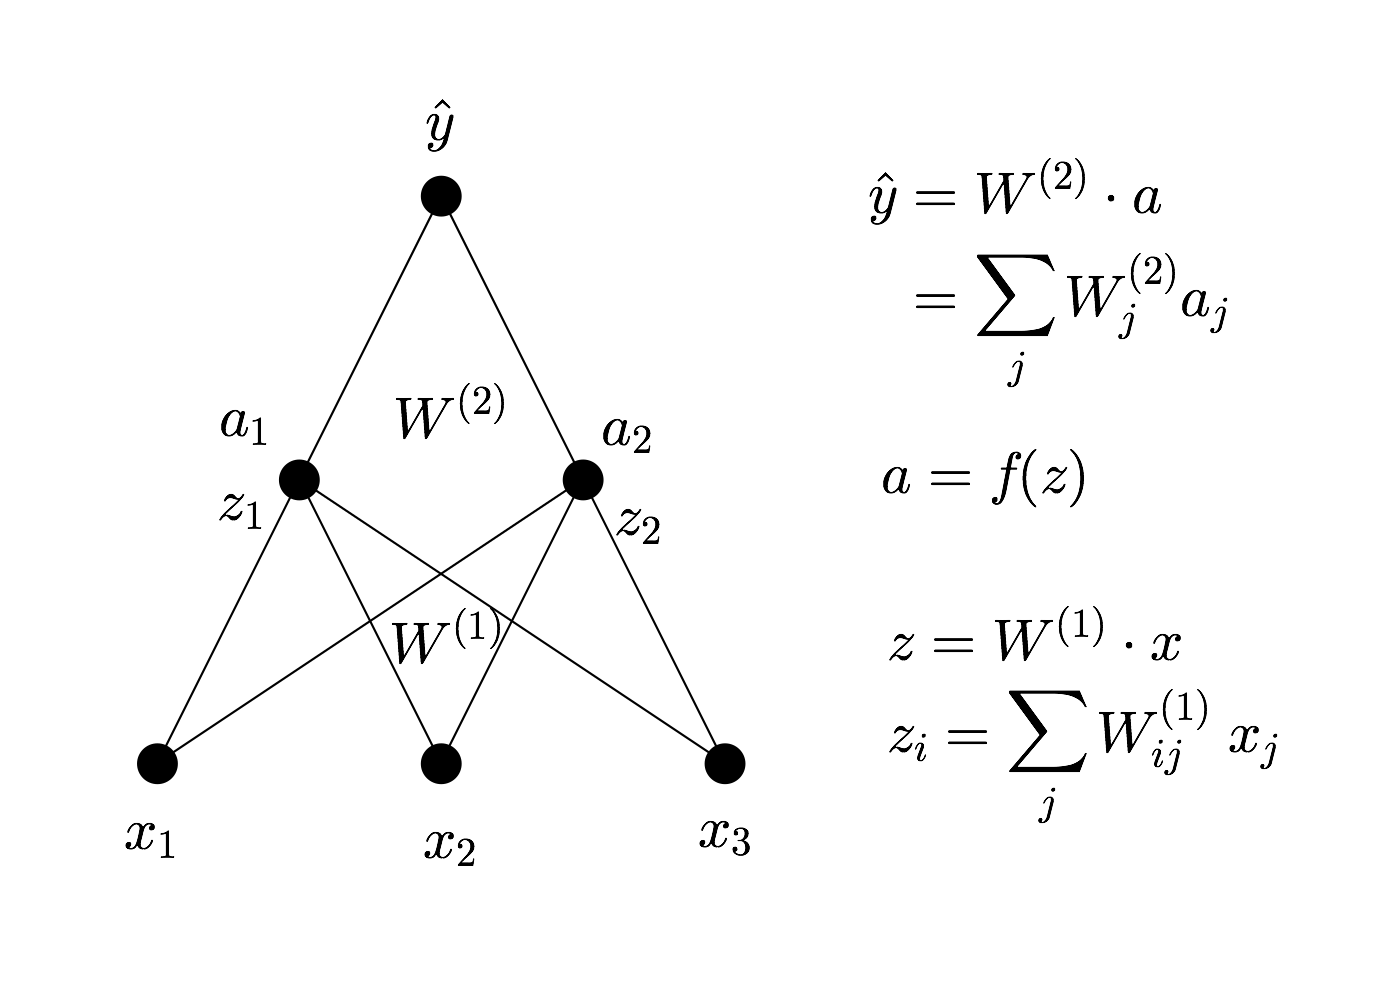
\includegraphics[scale=0.2]{neuralnet.png}
     \caption{\emph{Feedforward on a Neural Net} }
     \label{mandel2}
\end{figure}
\pagebreak
 \subsection{Feedforward}

Let $x$ be an $n$-dimensional vector encoding an example data point and let $y$ be its target. How do we calculate the output of the neural net? Step by step:
\begin{itemize}
\item The inputs to the hidden layer are encoded in the components of a $m$-dimensional column vector $z = W^{(1)} \cdot x$. The first component is the input to the first node, the second to the second and so on.
\item Each neurone in the hidden layer transforms the inputs, which are a linear combination of the features $x$ into an output, via the activation function: $a_i = f(z_i)$ or in shorthand $a = f(z)$.
\item Finally, the activations of the hidden layer are combined in the output: $\hat y = W^{(2)} \cdot a$.
\end{itemize}

\subsection{Cost Function}

In gradient descent, we want to modify the weights in order to get better and better predictions. How do measure the success of the network on a certain dataset? Consider a set of $L$ examples and targets $(x^{(l)},y^{(l)})$. We can measure the performance of the neural network by calculating the average square error:
\begin{equation}
E = \frac{1}{2L}\sum_{l =1}^{L}\left(y^{(l)}- \hat y^{(l)}\right)^2
\end{equation}
The smaller the error, the better the prediction\footnote{I snuck in a factor of $1/2$ because it makes the formulas easier to read. Why is this not a problem?}.

We can now calculate the gradient of $E$ with respect to the weights, and modify them so that the next time we make predictions, the error is smaller\footnote{If you do not understand this, you need to brush up on partial derivatives, go to Section \ref{grads}.}.
\pagebreak
\subsection{Backpropagation}

Calculating the gradients is just a matter of partial differentiation. I recommend reading this, copying the diagram and doing it without reading. Let's go!     
 
Let's start by calculating the partial derivatives with respect to the elements of $W^{(2)}$:
\begin{align}
\frac{\partial E~}{\partial W^{(2)}_i} 
&=  \frac{1}{2L}\sum_{l =1}^{L} \frac{\partial ~}{\partial W^{(2)}_i} \left(y^{(l)}- \hat y^{(l)}\right)^2 
&
&\mbox{past the sum}
\\[10pt] 
&=   \frac{1}{L}\sum_{l =1}^{L} -\left(y^{(l)}- \hat y^{(l)}\right) \frac{\partial  \left(y^{(l)}- \hat y^{(l)}\right)}{\partial W^{(2)}_i}
&
&\mbox{chain rule}
\\[10pt]
&=   \frac{1}{L}\sum_{l =1}^{L} \left(y^{(l)}- \hat y^{(l)}\right) \frac{\partial \hat y^{(l)}}{\partial W^{(2)}_i}
&
&y^{(l)} \mbox{ does not depend on the weights}\label{pa}
\\[10pt]
&=   \frac{1}{L}\sum_{l =1}^{L} \left(y^{(l)}- \hat y^{(l)}\right)  a_i^{(l)} 
&
&\mbox{by (\ref{linear}), since } \hat y^{(l)} = W^{(2)} \cdot a^{(l)} \label{grad2}
\end{align}
This is our first gradient! Notice that even though we think of $a^{(l)}$ as a column vector, the gradient needs to be of the same shape as $W^{(2)}$, since it tells us in which direction $E$ changes the fastest when we change $W^{(2)}$. While (\ref{grad2}) is the correct component wise formula, in linear algebra we could write:
\begin{equation}
\nabla_{W^{(2)}} E= \frac{1}{L}\sum_{l =1}^{L} \left(y^{(l)}- \hat y^{(l)}\right)  {a^{(l)}}^T 
\end{equation}      
Time to do the partial derivatives of $E$ with respect to the components of $W^{(1)}$. Notice this time we have two indices per component, whereas until now, each variable had only one index. This does not change the way we think of partial differentiation: when we take the partial with respect to a particular component, we treat the others as constants. For the Kronecker delta, we will write\footnote{Check that this works as intended!}:
\[
\frac{\partial{W_{ij}^{(1)}}}{\partial{W_{kd}^{(1)}}} = \delta_{ik}\delta_{jd}
\]
Let's go! The beginning looks just like before.
\begin{align}
\frac{\partial E~}{\partial W^{(1)}_{ij}} 
&=  \frac{1}{2L}\sum_{l =1}^{L} \frac{\partial ~}{\partial W^{(1)}_{ij}} \left(y^{(l)}- \hat y^{(l)}\right)^2 
&
&\mbox{past the sum}
\\[10pt] 
&=   \frac{1}{L}\sum_{l =1}^{L} -\left(y^{(l)}- \hat y^{(l)}\right) \frac{\partial  \left(y^{(l)}- \hat y^{(l)}\right)}{\partial W^{(1)}_{ij}}
&
&\mbox{chain rule}
\\[10pt]
&=   \frac{1}{L}\sum_{l =1}^{L} \left(y^{(l)}- \hat y^{(l)}\right) \frac{\partial \hat y^{(l)}}{\partial W^{(1)}_{ij}}
&
&y^{(l)} \mbox{ does not depend on the weights}\label{pa}
\end{align}
Let's focus on the partial derivative:
\begin{align}
\frac{\partial \hat y^{(l)}}{\partial W^{(1)}_{ij}}
&= \frac{\partial~}{\partial W^{(1)}_{ij}}\sum_k W_k^{(2)} f(z_k^{(l)})
&
&\mbox{substitution}
\\[10pt]
&= \sum_k \frac{\partial~}{\partial W^{(1)}_{ij}}  W_k^{(2)} f(z_k^{(l)})
&
&\mbox{past the sum}
\\[10pt]
&= \sum_k  W_k^{(2)}  \frac{\partial~}{\partial W^{(1)}_{ij}}f(z_k^{(l)})
&
&W_k^{(2)} \mbox{ is kept constant}
\\
&=  \sum_k  W_k^{(2)} f'(z_k^{(l)})  \frac{\partial z_k^{(l)}}{\partial W^{(1)}_{ij}}
&
&\mbox{chain rule}
\\[10pt]
&=  \sum_k  W_k^{(2)} f'(z_k^{(l)})\frac{\partial ~}{\partial W^{(1)}_{ij}}
\sum_d W^{(1)}_{kd}x_d^{(l)}
&
&\mbox{substitution}
\\[10pt]
&=  \sum_k  W_k^{(2)} f'(z_k^{(l)})
\sum_d x_d^{(l)} \frac{\partial W^{(1)}_{kd}}{\partial W^{(1)}_{ij}}
&
&x_d\mbox{ does not depend on } W^{(1)}
\\[10pt]
&=  \sum_k  W_k^{(2)} f'(z_k^{(l)}) \sum_d x_d^{(l)} \delta_{ki}\delta_{dj}
&
&\mbox{finally the Kronecker deltas!}
\\[10pt]
&=  \sum_k  W_k^{(2)} f'(z_k^{(l)}) x_j^{(l)} \delta_{ki}
&
&\mbox{sum over } d
\\[10pt]
&=   W_i^{(2)} f'(z_i^{(l)}) x_j^{(l)}
&
&\mbox{sum over } k
\end{align}
We can now pop back where we left off:
\begin{align}
\frac{\partial E~}{\partial W^{(1)}_{ij}} 
&=   \frac{1}{L}\sum_{l =1}^{L} \left(y^{(l)}- \hat y^{(l)}\right) \frac{\partial \hat y^{(l)}}{\partial W^{(1)}_{ij}}
&
&
\\[10pt]
&= \frac{1}{L}\sum_{l =1}^{L} \left(y^{(l)}- \hat y^{(l)}\right)  W_i^{(2)} f'(z_i^{(l)}) x_j^{(l)}
&
&
\end{align}
And we are done! Algebraically, we could sum all these equations with:
\begin{equation}
\nabla_{W^{(1)}} E= \frac{1}{L}\sum_{l =1}^{L} \left(y^{(l)}- \hat y^{(l)}\right)  \left(W^{(2)}*f'(z^{(l)})^T\right)\cdot x^{(l)}
\end{equation}  
where $*$ represents element-wise multiplication.       

We went pretty deep, but each step is simple and it's a matter of keeping track carefully of what you are differentiating, what is kept constant and what \emph{is} a constant. In this case, both the $x^{(l)}$ and the $y^{(l)}$ are constants, since they come from our database. It is good to recognise that the weights are indeed, all together at the same time, the variables of the cost function $E$.

Once we have the formulas for the gradients, it is easier to see what we need to calculate. Hopefully, by looking at the below, you can tell why it is called backpropagation, and by understanding the derivation, you can understand why backpropagation can give us the gradients.

\begin{figure}[h]
	\centering
     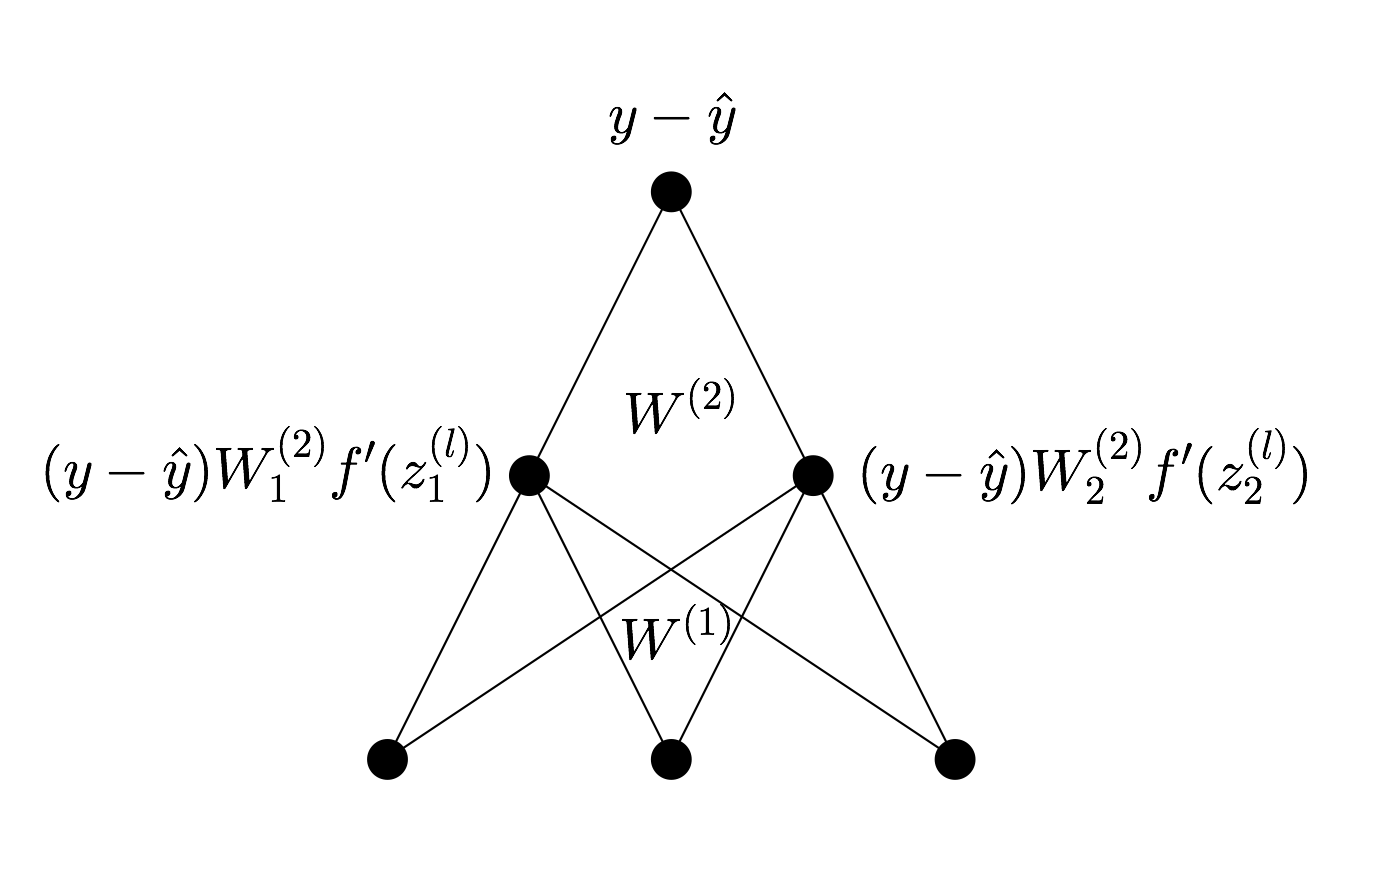
\includegraphics[scale=0.2]{neuralnet2.png}
     \caption{\emph{Errors on a Neural Net} }
     \label{mandel2}
\end{figure}


\end{document}  